% Campaign paper for vertical-cloud-lab/digital-alloy-lab#277. Due 28 Feb 2027.
% Build:  make        (draft: placeholders in red, notes shown)
%         make clean-pdf  (placeholders still shown, notes hidden)
% Numbers, tables and figures that depend on campaign data are generated by
% ../scripts/make_figures.py into generated/ and figures/. Do not type them in by hand.
\documentclass[preprint,12pt]{elsarticle}

\usepackage[T1]{fontenc}
\usepackage{lmodern}
\usepackage{amsmath,amssymb}
\usepackage{graphicx}
\usepackage{booktabs}
\usepackage{siunitx}
\usepackage{xcolor}
\usepackage[hidelinks]{hyperref}
\usepackage{lineno}
\usepackage{textcomp}
\usepackage{xspace}

\sisetup{detect-all, range-phrase = --, range-units = single, product-units = single}

% ---- draft toggles ---------------------------------------------------------
\ifdefined\cleanbuild
  \newcommand{\note}[1]{}
\else
  \newcommand{\note}[1]{\textcolor{blue!70!black}{\textsf{\footnotesize [Note: #1]}}}
  \linenumbers
\fi
% A value the campaign has not produced yet. Always visible, so nothing is submitted with one left in.
\newcommand{\placeholder}[1]{\textcolor{red!75!black}{[#1]}}
\newcommand{\Scal}{Scalmalloy\xspace}
\newcommand{\AlSi}{AlSi10Mg\xspace}

% Generated by scripts/make_figures.py. Do not edit by hand.
\newcommand{\InhouseYS}{228}
\newcommand{\InhouseYSsd}{13}
\newcommand{\InhouseYShw}{21}
\newcommand{\InhouseUTS}{376}
\newcommand{\InhouseUTSsd}{10}
\newcommand{\InhouseEL}{4.5}
\newcommand{\InhouseELsd}{0.5}
\newcommand{\InhouseN}{4}
\newcommand{\NAlRuns}{\placeholder{N runs}}
\newcommand{\NCompositions}{\placeholder{N compositions}}
\newcommand{\BAlSinir}{\placeholder{B}}
\newcommand{\BAlSicost}{\placeholder{B}}
\newcommand{\BScalnir}{\placeholder{B}}
\newcommand{\BScalcost}{\placeholder{B}}


\journal{\placeholder{Additive Manufacturing Letters (version A) or Additive Manufacturing (version B); see ../journals.md}}

\begin{document}

\begin{frontmatter}

\title{\placeholder{Version A:} A scandium-free aluminum alloy for laser powder bed fusion (PBF-LB/M) that is stronger than \AlSi at equal ductility}

\author[byu]{\placeholder{Co-authors to confirm}}
\author[byu]{Sterling G. Baird\corref{cor}}
\cortext[cor]{Corresponding author}
\affiliation[byu]{organization={Brigham Young University},
  city={Provo}, state={UT}, country={USA}}

\begin{abstract}
\placeholder{Write at G4 (29 Jan); length per ../journals.md.}
\AlSi, the most widely printed aluminum alloy for laser powder bed fusion (PBF-LB/M), is easy to print but modest in strength, while \Scal reaches about 1.5 to 2.1 times its yield strength by adding scandium, a critical mineral that the United States imports entirely.
We ran a 12-week campaign to find a printable alloy that is stronger than \AlSi without scandium.
CALPHAD screening ranked \placeholder{N\textsubscript{screen}} scandium-free compositions on solidification range, crack susceptibility, strengthening phases and a critical-mineral burden fixed before the screen; \NCompositions{} were atomized in-house from dosed \SI{250}{g} charges, printed by PBF-LB/M, and tested for density, hardness, tensile properties and corrosion in \SI{3.5}{wt\%} NaCl.
\placeholder{Version A: Alloy X (Al--\dots) printed crack-free to \dots\% density and reached \dots~MPa yield strength and \dots\% elongation, \dots~MPa above \AlSi printed and tested the same way, with a critical-mineral burden \dots\% below \Scal's. An outside laboratory confirmed its composition.}
\placeholder{Version B: \dots}
\end{abstract}

\begin{keyword}
laser powder bed fusion (PBF-LB/M) \sep aluminum alloys \sep scandium-free \sep critical minerals \sep ultrasonic atomization \sep CALPHAD
\end{keyword}

\end{frontmatter}


\note{Highlights (Elsevier: 3--5 bullets, at most 85 characters each, separate file). Drafts, to be fixed at G4: (1) Scandium-free Al alloy [X] printed crack-free from in-house powder. (2) [YS] MPa yield, above AlSi10Mg printed and tested the same way. (3) Critical-mineral burden [X]\% below Scalmalloy on a metric fixed in advance. (4) [N] compositions atomized and tested in 12 weeks.}

% =============================================================================
\section{Introduction}
\label{sec:intro}

Laser powder bed fusion (LPBF; PBF-LB/M in ISO/ASTM 52900 terms) can build thin-walled, topology-optimized aluminum parts that are hard to cast or machine, and aluminum's low density makes those parts attractive for aircraft, launch vehicles and satellites~\cite{debroy2018,aboulkhair2019,kotadia2021}.
Most aluminum alloys used in LPBF were not designed for it.
The workhorse, \AlSi, is a near-eutectic casting alloy: its short freezing range makes it easy to print without cracks, but its strength is modest, and the heat treatments that restore ductility cost strength (Section~\ref{sec:benchmark})~\cite{aboulkhair2019,ds_eos,ds_nikon}.
The high-strength wrought alloys of the 2xxx and 7xxx series, by contrast, crack as they solidify in LPBF unless their grain structure is refined~\cite{martin2017,kou2015}.

\Scal, an Al--Mg--Sc--Zr alloy, shows what an alloy designed for the process can do.
Al\textsubscript{3}(Sc,Zr) particles that form in the melt nucleate fine equiaxed grains at the melt-pool boundaries, which suppresses hot cracking, and the same elements precipitate as nanoscale L1\textsubscript{2} particles on aging~\cite{spierings2017}.
After a direct age at \SI{325}{\celsius} it reaches \SIrange{465}{500}{MPa} yield strength with \SIrange{11.5}{15.8}{\%} elongation on vendor datasheets~\cite{ds_colibrium,ds_3dsystems}, about 1.5 to 2.1 times the \SIrange{233}{300}{MPa} of as-built \AlSi~\cite{ds_eos,ds_nikon}.
Its weakness is scandium.
Scandium is recovered only as a byproduct, world production in 2025 was about 80~t (scandium oxide equivalent), the United States relied on imports for all of its supply, and China, the leading producer, placed scandium metal, alloys and compounds under export control in April 2025~\cite{usgs2026sc}; scandium is on the final 2025 U.S.\ List of Critical Minerals~\cite{fr2025}, and U.S.\ strategy treats lowering demand for such materials as a goal in its own right~\cite{doe2023}.
An alloy that is stronger than \AlSi without scandium, or as strong as \Scal with less of it, would remove a supply risk from a growing class of printed flight hardware.

Scandium-free routes to printable, high-strength aluminum already exist.
In Al--Mg--Zr alloys, primary L1\textsubscript{2} Al\textsubscript{3}Zr particles refine the grains, and nanoscale Al\textsubscript{3}Zr precipitates formed on aging raise the strength by more than 40\%~\cite{croteau2018}.
Inoculant particles added to the powder suppress cracking in 7075 and 6061~\cite{martin2017,opprecht2020}.
Al--Mn--Cr--Zr-based alloys designed for LPBF~\cite{almncr2022,alloyF2024} reach about \SI{390}{MPa} yield strength as built~\cite{almncrzr2024}, Al--Mg--Mn--Er--Zr alloys about \SI{440}{MPa} after aging~\cite{almgmnerzr2022}, and Al--Ce--Mn alloys keep their strength to high temperature~\cite{plotkowski2020}.
Several scandium-free powders are now sold for LPBF: Al--Mn--Cr--Zr and Al--Mg--Zr--Mn grades with datasheet yield strengths well above \AlSi's after a direct age, and an Al--Fe--Zr grade that matches it~\cite{ds_hoganas,ds_al5x1,ds_cp1}.
Computational design has produced printable alloys too: by CALPHAD-based integrated computational materials engineering~\cite{thapliyal2020} and by CALPHAD coupled with Bayesian optimization~\cite{taherimousavi2025}, although with scandium or rare-earth additions, and by CALPHAD-aided design of a crack-free Al--Mg--Si--Ti alloy refined by Al$_3$Ti, with neither~\cite{wen2024}.
Two problems remain.
First, few of these alloys have been compared with \AlSi printed and tested in the same way~\cite{alsimg2020}, so whether an alloy is ``better'' depends on which datasheet it is compared with (Fig.~\ref{fig:map}a, Section~\ref{sec:benchmark}).
Second, removing scandium does not by itself reduce the critical-mineral burden. The final 2025 U.S.\ list includes aluminum and silicon themselves, as well as Mg, Mn, Cr, Zr, Ti, Cu, Ni and the rare earths; of the elements used in these alloys, only iron is absent~\cite{fr2025}. A claim of ``less critical minerals'' therefore needs a burden metric that weights each element, stated in advance~\cite{graedel2012,mulukutla2025}.

\begin{figure}[tbp]
  \centering
  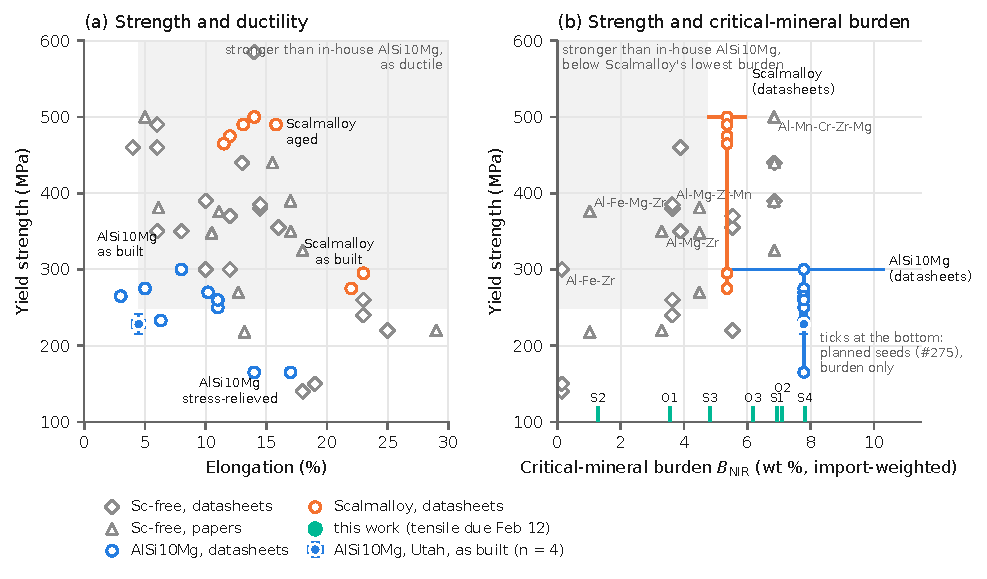
\includegraphics[width=\textwidth]{figures/fig1-benchmark-map.pdf}
  \caption{Where the campaign's alloys sit against the benchmarks. (a) Yield strength against elongation. Open blue and orange markers, \AlSi and \Scal vendor datasheets~\cite{ds_eos,ds_nikon,ds_colibrium,ds_3dsystems}; filled blue, \AlSi printed for this work at the University of Utah (as built, as-printed surfaces, horizontal; mean $\pm$ s.d., $n=\InhouseN$); grey diamonds, scandium-free alloys on vendor datasheets~\cite{ds_hoganas,ds_al5x1,ds_cp1,ds_a20x,ds_7a77,ds_al2139}; grey triangles, scandium-free alloys in papers~\cite{almncrzr2024,croteau2018,almgmnerzr2022,alfezr2025,alsimg2020}; dashed grey boxes, scandium-free alloys whose datasheets give only a range; grey shading, where a candidate's mean must lie to be stronger than our \AlSi at no lower elongation (the rule of Section~\ref{sec:stats} also adds the candidate's own confidence half-width). (b) Yield strength against the import-weighted burden $B_\mathrm{NIR}$ (Eq.~\ref{eq:burden}), plotted at the midpoint of its interval; the horizontal bars on the benchmarks show the interval. Green ticks mark the burden of the planned seed compositions, whose strength is not yet measured. Shading: stronger than our \AlSi and below the lower end of \Scal's burden; the scandium-free values are as reported, mostly on machined specimens, so they are not like-for-like with ours. \placeholder{Campaign alloys (green dots) are added as their tensile data arrive.}}
  \label{fig:map}
\end{figure}

The slower problem is powder.
Every new composition needs its own powder, and gas atomization, the usual route, runs at a scale and lead time suited to production rather than exploration~\cite{anderson2018}.
Blending elemental powders and alloying them in the melt pool avoids atomization, but leaves compositional inhomogeneity and unmelted particles~\cite{mosallanejad2021}.
Ultrasonic atomization melts a charge of a few hundred grams or less and breaks the melt into near-spherical droplets on a vibrating surface, which makes one powder per candidate practical~\cite{zrodowski2021,priyadarshi2024}; the same route made the powder for a recently designed high-strength alloy~\cite{taherimousavi2025}.

Here we report a 12-week campaign that puts these pieces together.
We screened \placeholder{N\textsubscript{screen}} scandium-free compositions with CALPHAD for freezing range, crack susceptibility, strengthening phases and a critical-mineral burden that was fixed before the screen ranked anything; atomized \NCompositions{} of them in-house from dosed charges; printed them by LPBF; and measured density, hardness, tensile properties and corrosion.
Each result is compared with \AlSi printed on the same machine and tested the same way, with vendor datasheets as context, and with \Scal on critical-mineral burden.
\placeholder{Version A: We find that \dots}
\placeholder{Version B: We find that \dots}

% =============================================================================
\section{Materials and methods}
\label{sec:methods}

\note{Methods are written for the plan in the \#256 schedule and the \#275 seed plan. Every bracket is a value to read off the run record, the SOP (\#253) or the instrument, not to estimate. Delete any subsection whose step does not happen.}

\subsection{Design space and CALPHAD screening}
\label{sec:calphad}

Compositions were drawn from the lab's elemental palette (Al with Mn, Cr, Zr, Mg, Si, Cu, Ti, Fe, Ni, Ce, Li, Er, Zn and Sn) with scandium excluded, Al $\geq$ \placeholder{85}~wt\%, and the bounds in Supplementary Section~S2.
\note{The kickoff (11:29) suggested keeping Si out unless composition can be verified for Si-bearing alloys. Spark-OES (ASTM E1251) on a printed coupon avoids the digestion problem; decide before the screen.}
Equilibrium and Scheil--Gulliver solidification were computed for each composition with \placeholder{Thermo-Calc 202x with TCAL\,\dots, through TC-Python~\cite{andersson2002} / pycalphad~\cite{otis2017} with the MatCalc \texttt{mc\_al} and COST~507 databases}.
\note{No Thermo-Calc licence yet (\#141). The open-database screen cannot predict the Al\textsubscript{3}Zr liquidus (MatCalc mc\_al has none, per \#275), which matters for every Zr-bearing candidate. If Thermo-Calc arrives late, re-check the finalists in it and report both.}
Four quantities ranked the compositions:
(i) the freezing range, taken between the liquidus and a solid fraction of \placeholder{0.99} in the Scheil calculation;
(ii) Kou's index of crack susceptibility, $\lvert \mathrm{d}T / \mathrm{d}(f_\mathrm{s}^{1/2}) \rvert$ near $f_\mathrm{s}^{1/2} = 1$~\cite{kou2015};
(iii) the predicted mole fraction of strengthening phases (L1\textsubscript{2} Al\textsubscript{3}M and other precipitates) at the aging temperature, and whether a primary L1\textsubscript{2} phase forms ahead of the aluminum matrix during solidification, where it can act as a grain refiner~\cite{croteau2018,spierings2017}; and
(iv) the critical-mineral burden $B$ (Section~\ref{sec:burden}).
Printable laser settings for each candidate were estimated from Eagar--Tsai melt-pool calculations and printability maps that bound lack of fusion, balling and keyholing~\cite{eagar1983,johnson2019}.

Four seed compositions spanning distinct strengthening routes (S1--S4 in Table~\ref{tab:compositions}, with three optional ones) were atomized first.
\note{The \#275 plan proposes S1 Al--4.8Mn--0.9Cr--1.1Zr--1.2Mg, S2 Al--1.9Fe--1.0Mg--1.0Zr, S3 Al--3.5Si--2.5Mg and S4 Al--6Mg--2.5Si--0.7Ti, chosen from the literature, not from the screen. If they stay, say so plainly here: they are literature anchors, and the screen ranks what follows.}
Later compositions were proposed in batches of three by Bayesian optimization~\cite{balandat2020} on the measured hardness and relative density, with the CALPHAD quantities as inputs; the settings were fixed before the first round (Supplementary Section~S9). The software that schedules the steps of the loop, in the manner of a self-driving laboratory~\cite{tom2024}, is described elsewhere~\placeholder{ref.\ to the \textit{Adv.\ Mater.} article, if out first}; here it serves only to pick compositions.
\note{Keep the optimizer to this paragraph. The cost-aware network optimizer and any acceleration claim belong to the \textit{Adv.\ Mater.} article (\#120); see ../outline.md.}

\begin{table}[tbp]
  \centering\footnotesize
  \caption{Nominal compositions (wt\%, balance Al) and critical-mineral burden. $B_\mathrm{NIR}$: import-weighted burden (Eq.~\ref{eq:burden}); $B_\mathrm{cost}$: raw-material cost of the alloying additions. \placeholder{Measured compositions (EDS in-house, ICP-OES outside) are added for the campaign alloys.}}
  \label{tab:compositions}
  \resizebox{\textwidth}{!}{\begin{tabular}{@{}lrrr@{}}
\toprule
Alloy & $B_\mathrm{NIR}$ & $B_\mathrm{cost}$ & Sc \\
 & wt\% & USD\,kg$^{-1}$ & wt\% \\
\midrule
AlSi10Mg & -- & -- & -- \\
Scalmalloy & -- & -- & -- \\
\midrule
\multicolumn{4}{@{}l}{\placeholder{Campaign alloys with measured compositions: due Feb 19, 2027}} \\
\bottomrule
\end{tabular}
}
\end{table}

\subsection{Critical-mineral burden}
\label{sec:burden}

The burden of an alloy was computed from its composition as
\begin{equation}
  B_\mathrm{NIR} = \sum_{i \neq \mathrm{Al}} w_i \, \frac{\mathrm{NIR}_i}{100},
  \label{eq:burden}
\end{equation}
where $w_i$ is the mass fraction of alloying element $i$ in wt\% and $\mathrm{NIR}_i$ is the U.S.\ net import reliance for that element in 2025, as a percentage of apparent consumption~\cite{usgs2026}.
$B_\mathrm{NIR}$ is a mass fraction of the alloying additions, in wt\% of the alloy, with each element weighted by the share of U.S.\ supply that is imported on balance; it is a measure of import exposure, not of where a given batch was sourced.
Aluminum is left out because it is the base of every alloy compared (Supplementary Section~S3 shows what counting it does), and iron, which is not on the 2025 list and of which the U.S.\ is a net exporter, counts as zero.
USGS reports some reliances only as bounds (silicon above 50\%, magnesium above 75\%, zirconium below 25\%), so $B_\mathrm{NIR}$ is reported as the interval those bounds allow, and plotted at its midpoint.
As sensitivity checks we report the raw-material cost of the critical alloying additions per kilogram of alloy, $B_\mathrm{cost} = \sum (w_i/100)\,p_i$ over the elements on the 2025 list other than aluminum, with 2025 prices $p_i$ (2023 for manganese metal, which USGS no longer prices; scandium as metal)~\cite{usgs2026}, and the scandium content alone.
The inputs and their sources are in Supplementary Section~S3.
The metric, its inputs and the threshold for ``less than \Scal'' were committed to the project repository before the CALPHAD screen ranked any composition (Supplementary Section~S9).
\note{Sterling to choose the primary metric and the threshold. FLAIME's O4 uses $\geq$40\% below \Scal. Check how the seeds score before freezing: an Al--Mn--Cr--Zr alloy carries several wt\% of fully imported Mn (risks.md, R7).}

\subsection{Feedstock and charges}

Each \SI{250}{g} charge was made from \placeholder{6063 aluminum bar from a single lot (\dots)}, with Si from 4047 rod, Zr from an Al--10Zr master alloy and the other additions as elemental metal \placeholder{(purities and suppliers)}.
Masses were weighed to \placeholder{$\pm$0.01~g} and the target composition was computed from the masses and the certified composition of each feedstock, including the 6063 base (about \SI{0.5}{wt\%} Mg, \SI{0.35}{wt\%} Si and \SI{0.2}{wt\%} Fe).
Mg was over-charged by \placeholder{5--10\%} to offset evaporation until the first outside analysis gave a measured loss.

\subsection{Ultrasonic atomization}
\label{sec:atomization}

Powders were made in an ultrasonic atomizer (rePOWDER, AMAZEMET) with an induction-heated crucible.
The charge was melted under argon after \placeholder{three} evacuation and backfill cycles, with chamber O\textsubscript{2} below \placeholder{20}~ppm before heating; held for \placeholder{2}~min at a set point of the highest calculated liquidus plus \SI{100}{\celsius} and at least \SI{820}{\celsius}; and poured through a \placeholder{boron nitride} nozzle under \placeholder{0.19}~bar argon overpressure onto a molybdenum plate vibrating at \placeholder{40}~kHz, driven through a 1.5:1 booster at \placeholder{90}\% amplitude.
Settings other than the melt temperature were the same for every run and follow the lab's operating procedure \placeholder{(SOP version and commit)}.
Every run was recorded on video, and its settings, masses and outcome were logged in the run table (Supplementary Section~S1), including runs that failed.

\subsection{Powder handling and characterization}

Within \SI{48}{h} of each run, the powder was weighed and sieved on a sieve set used only for aluminum, at \SIlist{250;63}{\micro m} \placeholder{and 45~\textmu m}~\cite{astm_b214}; the fraction below \SI{63}{\micro m} was used for LPBF.
Powders were stored sealed with desiccant at below \placeholder{X}\% relative humidity, and dried at \SI{80}{\celsius} for \SI{4}{h} before printing.
Particle size and shape were measured by SEM image analysis of at least 1000 particles (size) and 400 particles (shape) per lot, following ISO 13322-1 and ISO 9276-6~\cite{iso13322,iso9276}.
Composition was measured in-house by standards-based SEM--EDS on polished powder cross-sections \placeholder{(instrument, kV, standards, DTSA-II)} and, for the benchmarks and finalists, by an outside laboratory (Section~\ref{sec:verification}).
A sealed \SI{5}{g} sample of each lot was kept for oxygen analysis.

\subsection{Laser powder bed fusion}
\label{sec:lpbf}

Specimens were printed on an Aconity MIDI at the University of Utah \placeholder{(build plate material, preheat \textdegree C, argon, O\textsubscript{2} below \dots~ppm, reduced build platform if used)}.
Each composition was printed first as single tracks, then as 5\,$\times$\,5\,$\times$\,5~mm cubes over a matrix of \placeholder{2} powers $\times$ \placeholder{4} speeds $\times$ \placeholder{2} hatch spacings at \placeholder{50}~\textmu m layers with a \SI{67}{\degree} rotation between layers, and finally as tensile specimens at the setting that gave the highest density.
Tensile specimens were flat ASTM E8/E8M sub-size specimens (\SI{100}{mm} long, \SI{6}{mm} wide and \SI{6}{mm} thick in the reduced section, \SI{32}{mm} reduced length)~\cite{astm_e8}, built flat (horizontal), the same geometry and orientation as the \AlSi reference build of April 2026.
\note{The April coupons' dimensions (PR \#288) match the E8/E8M sub-size outline, but the project records don't call them E8 sub-size; confirm against the drawing in \#138 before saying so.}
To separate the effect of the alloy from that of the powder route, the finalists' build also contained \AlSi-type powder atomized in-house (run D1) and commercial gas-atomized \AlSi powder, printed with \placeholder{the same / their own optimized} parameters.

\subsection{Heat treatment}

\AlSi specimens were tested as built and after a stress relief at \placeholder{\SI{300}{\celsius} for \SI{2}{h}}.
Each candidate was tested as built and after one direct-aging treatment chosen before printing from the CALPHAD precipitation calculations and the literature for its family; direct aging, without a solution treatment, can work because PBF-LB/M leaves a supersaturated matrix, as shown for a Mg$_2$Si-rich Al alloy~\cite{solanki2026} \placeholder{(e.g.\ \SI{400}{\celsius}, \dots~h for Zr-bearing alloys~\cite{croteau2018})}.

\subsection{Density, microstructure and hardness}

Relative density was measured by Archimedes' method~\cite{astm_b962} in \placeholder{water / ethanol} with \placeholder{three} repeats per cube, and checked by image analysis of polished sections.
Cracks and pores were examined on sections parallel to the build direction by optical microscopy and SEM.
Vickers microhardness was measured on polished sections~\cite{astm_e384} at \placeholder{HV0.5} with \placeholder{10} indents per condition.
Hardness was the optimizer's fast screen for strength; it was not converted to yield strength, because hardness--yield relations for aluminum alloys depend on work hardening and differ between alloys and tempers~\cite{tiryakioglu2015}.

\subsection{Tensile testing}

Tensile tests were run at room temperature on a \placeholder{20~kip / 100~kip} load frame at \placeholder{strain rate}, with strain measured by \placeholder{a clip-on extensometer / DIC} over a \SI{25}{mm} gauge length~\cite{astm_e8}.
The 0.2\% offset yield strength was taken from the extensometer; elongation after fracture from gauge marks.
Specimens that broke outside the gauge length were excluded and reported.
\note{The April 2026 \AlSi tests 1--3 gave elastic slopes of 29--49~GPa (aluminum is about 70~GPa), so their yield strengths are uncertain by up to about 30~MPa (PR \#288). The campaign tests need an extensometer.}

\subsection{Corrosion}

Corrosion was measured in aerated \SI{3.5}{wt\%} (\SI{0.6}{M}) NaCl at room temperature in a three-electrode cell \placeholder{(EZstat-Pro potentiostat, NuVant Systems; CubXL cell)} with an Ag/AgCl reference electrode and a \placeholder{graphite / platinum} counter electrode, on polished sections of printed cubes with an exposed area of \placeholder{X}~cm\textsuperscript{2}.
After \SI{30}{min} at open circuit, linear polarization resistance was measured over $\pm$\SI{10}{mV} at \SI{0.167}{mV\per s}, adapted from ASTM G59~\cite{astm_g59}, followed by a cyclic potentiodynamic scan following the procedure of ASTM G61, which is written for iron-, nickel- and cobalt-based alloys~\cite{astm_g61}; the corrosion current density was obtained by Tafel extrapolation and converted to a rate~\cite{astm_g102}, and the pitting potential was read from the anodic branch.
Printed \AlSi corrodes selectively along melt-pool boundaries, and heat treatment changes how it corrodes~\cite{cabrini2016,revilla2017,rubben2019}, so it was tested in the same condition as each candidate. Three specimens were tested per alloy and condition, alongside printed \AlSi and wrought 6063, and the set-up was first checked against \placeholder{a reference measurement~\cite{astm_g5}}.
\note{The instrument has so far passed dummy-cell checks only (PR \#239), EZware caps the open-circuit step at 20~min, and only one reference electrode is on order (PR \#264).}

\subsection{Independent verification}
\label{sec:verification}

The compositions of the benchmark powders and of the finalists' powders and printed parts were measured by \placeholder{an accredited outside laboratory} using ICP-OES~\cite{astm_e3061} and \placeholder{spark-OES on printed coupons~\cite{astm_e1251}}, and their oxygen content by inert-gas fusion.
Samples were sent under coded IDs, and the laboratory's results and uncertainties are reported as received.
\placeholder{If funded: tensile specimens from the finalists' build were also tested at an outside laboratory.}

\subsection{Statistics and the comparison with \AlSi}
\label{sec:stats}

Values are given as mean $\pm$ standard deviation with the number of valid specimens $n$; 95\% confidence intervals use Student's $t$.
A candidate was counted as stronger than \AlSi only if, printed on the same machine with the same specimen geometry and surface and tested the same way, its mean yield strength exceeded that of \AlSi by more than the half-widths of the two 95\% confidence intervals combined, with a mean elongation no lower than that of \AlSi and $n \geq 3$ for both.
This rule, and the choice of comparator, were fixed at the same time as the burden metric, before the screen ranked any composition (Supplementary Section~S9).

\subsection{Provenance}

Each powder lot has a record that links the charge, the atomizer settings and video, sieving, storage humidity, the print and every measurement to the file that holds it, in the format of Ref.~\placeholder{lot k7m2q9 record}.
The records, raw data and analysis code are listed in the Data and Code Availability statements.

% =============================================================================
\section{Results}
\label{sec:results}

\note{Every subsection below is a placeholder until its data exist. The dates are the figure plan's (../figure-plan.csv); ../figure-status.md shows what has been drawn.}

\subsection{Screen and selected compositions}
\placeholder{Data due 29 Jan 2027 (Fig.~\ref{fig:calphad}, Table~\ref{tab:compositions}).}
What the screen ranked highest; which compositions were made and why; where the optimizer's picks departed from the CALPHAD ranking.
A preliminary calculation with open databases for 48 compositions (Fig.~\ref{fig:calphad}): the nine planned seeds, 34 published alloys including seven known to crack, the 6063 base and four exploratory variants, already shows the pattern the screen has to handle. Alloys known to crack in LPBF, such as 2024, 6061 and 7075, sit at high crack index and wide freezing range; but so do the Scalmalloy-type and Al--Mg--Zr alloys, which print without cracks because a primary Al$_3$M phase refines their grains~\cite{spierings2017,croteau2018}. The crack index alone therefore cannot rank the Zr- and Sc-bearing candidates, and the screen weighs it together with the primary phase.
\note{Fig.~2 is drawn from the \#275 open-database calculations (MatCalc mc\_al, COST 507), not from the campaign screen, and the counts are of those rows; replace both when the screen runs. Kou's index is from the Scheil path, and COST 507 supplies the Al$_3$Zr liquidus that mc\_al lacks.}

\begin{figure}[tbp]
  \centering
  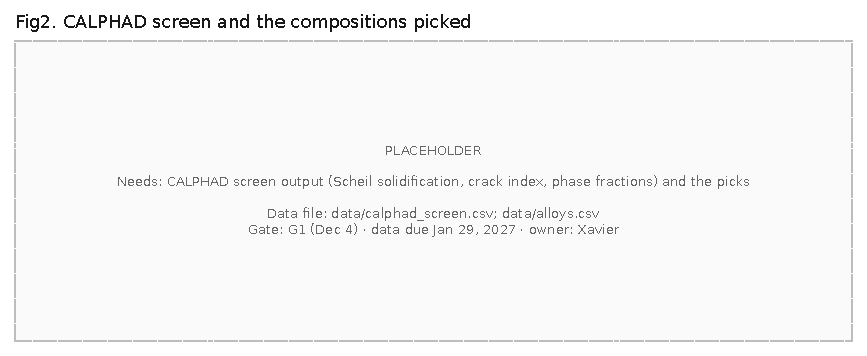
\includegraphics[width=\textwidth]{figures/fig2-calphad-screen.pdf}
  \caption{CALPHAD screen. (a) Kou's crack-susceptibility index near the end of solidification against the freezing range, from Scheil calculations with open databases (MatCalc mc\_al, with COST 507 for the Al$_3$Zr liquidus) on a pure-Al base, for the planned seeds (labelled), published scandium-free and Sc-bearing alloys, and alloys known to crack in LPBF (crosses). Filled markers have a primary Al$_3$M phase (M = Zr, Sc or Ti) that can refine the grains; colour is the import-weighted burden $B_\mathrm{NIR}$. \placeholder{Preliminary: to be replaced by the campaign's screen, with (b) the seeds and the optimizer's picks.}}
  \label{fig:calphad}
\end{figure}

\subsection{Powders}
\placeholder{Data due 12 Feb 2027 (Fig.~\ref{fig:powders}).}
Size and shape of each powder; how close the measured composition came to the target, and which elements were lost. Mn and Zn evaporated preferentially from the finest particles in an earlier ultrasonic-atomization study~\cite{zrodowski2021}, and Mg can be lost during LPBF at high energy input~\cite{croteau2018}. 

\begin{figure}[tbp]
  \centering
  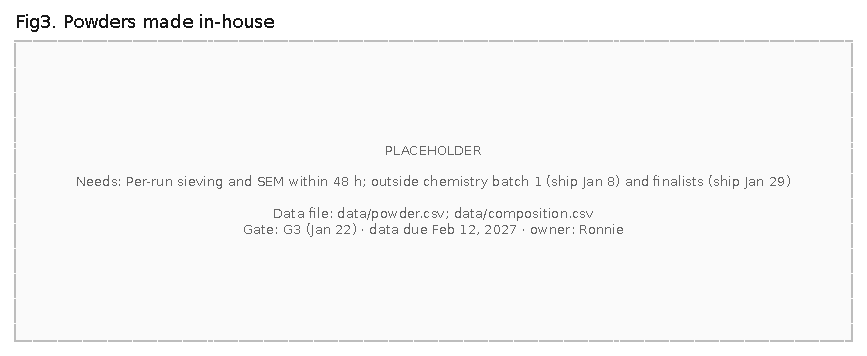
\includegraphics[width=\textwidth]{figures/fig3-powders.pdf}
  \caption{Powders made in-house. \placeholder{(a) SEM; (b) D10--D50--D90 and the fraction below 63~\textmu m; (c) measured against target composition.}}
  \label{fig:powders}
\end{figure}

\subsection{Printability}
\placeholder{Data due 5 Feb 2027 (Fig.~\ref{fig:print}).}
Which compositions printed crack-free and dense, and whether the CALPHAD crack index, together with the primary Al$_3$M phase (Section~3.1), predicted it.

\begin{figure}[tbp]
  \centering
  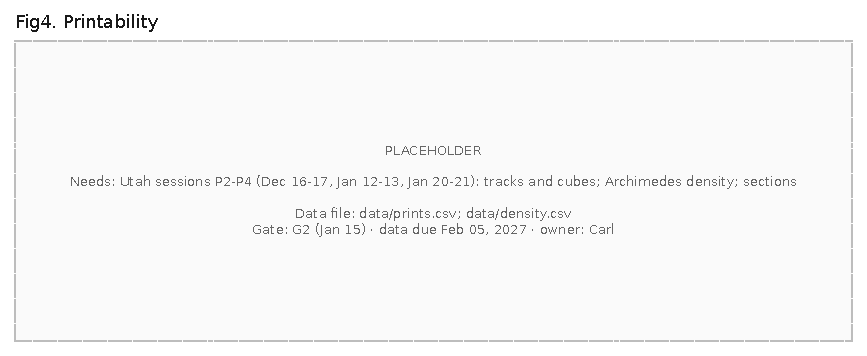
\includegraphics[width=\textwidth]{figures/fig4-printability.pdf}
  \caption{Printability. \placeholder{(a) Best relative density of each composition; (b) cracking against the CALPHAD crack index; (c) sections.}}
  \label{fig:print}
\end{figure}

\subsection{Strength and ductility}
\placeholder{Data due 12 Feb 2027 (Fig.~\ref{fig:mech}).}
The \AlSi reference printed at the University of Utah in April 2026 gave \InhouseYS~$\pm$~\InhouseYSsd~MPa yield strength, \InhouseUTS~$\pm$~\InhouseUTSsd~MPa tensile strength and \InhouseEL~$\pm$~\InhouseELsd\% elongation as built ($n = \InhouseN$; Fig.~\ref{fig:mech}c, Table~\ref{tab:benchmarks}). These tests used the load frame's own strain channel rather than an extensometer, so their yield strengths are uncertain by up to about 30~MPa (Section~\ref{sec:benchmark}).
\placeholder{Hardness of every printed composition; tensile results of the finalists and of in-house \AlSi-type powder from the same build.}

\begin{table}[tbp]
  \centering\footnotesize
  \caption{Room-temperature tensile properties of the two benchmarks. Datasheet values are vendor typical or mean values on machined bars, except the Nikon row marked as-printed surface, at \SIrange{30}{60}{\micro m} layers; the 3D Systems rows are at 30 and 60~\textmu m and give plastic elongation. The last row was measured for this work. \placeholder{Campaign rows are added by make\_figures.py as data arrive.}}
  \label{tab:benchmarks}
  \resizebox{\textwidth}{!}{\begin{tabular}{@{}llllrrr@{}}
\toprule
Alloy & Source & Condition & Orient. & YS (MPa) & UTS (MPa) & EL (\%) \\
\midrule
AlSi10Mg & EOS M 290~\cite{ds_eos} & as-built & vertical & 233 & 466 & 6.3 \\
AlSi10Mg & EOS M 290~\cite{ds_eos} & as-built & horizontal & 270 & 461 & 10.2 \\
AlSi10Mg & Nikon SLM 500~\cite{ds_nikon} & as-built & horizontal & 300 & 450 & 8.0 \\
AlSi10Mg & Nikon SLM 500~\cite{ds_nikon} & as-built & vertical & 275 & 470 & 5.0 \\
AlSi10Mg & Nikon SLM 500~\cite{ds_nikon} & as-built, as-printed surface & vertical & 265 & 425 & 3.0 \\
AlSi10Mg & EOS M 290~\cite{ds_eos} & EOS T6 & vertical & 250 & 310 & 11.0 \\
AlSi10Mg & EOS M 290~\cite{ds_eos} & EOS T6 & horizontal & 260 & 320 & 11.0 \\
AlSi10Mg & Nikon SLM 500~\cite{ds_nikon} & stress relief SR1 & horizontal & 165 & 280 & 17.0 \\
AlSi10Mg & Nikon SLM 500~\cite{ds_nikon} & stress relief SR1 & vertical & 165 & 285 & 14.0 \\
Scalmalloy & Colibrium M2~\cite{ds_colibrium} & as-built & horizontal & 295 & 355 & 23.0 \\
Scalmalloy & Colibrium M2~\cite{ds_colibrium} & as-built & vertical & 275 & 350 & 22.0 \\
Scalmalloy & Colibrium M2~\cite{ds_colibrium} & direct age 325 C 4 h & horizontal & 475 & 515 & 12.0 \\
Scalmalloy & Colibrium M2~\cite{ds_colibrium} & direct age 325 C 4 h & vertical & 465 & 505 & 11.5 \\
Scalmalloy & 3D Systems~\cite{ds_3dsystems} & 325 C 4 h air cool & horizontal & 490 & 520 & 15.8 \\
Scalmalloy & 3D Systems~\cite{ds_3dsystems} & 325 C 4 h air cool & vertical & 490 & 520 & 15.8 \\
Scalmalloy & 3D Systems~\cite{ds_3dsystems} & 325 C 4 h air cool & horizontal & 500 & 530 & 14.0 \\
Scalmalloy & 3D Systems~\cite{ds_3dsystems} & 325 C 4 h air cool & vertical & 490 & 520 & 13.1 \\
\midrule
Al-HS1 & H\"ogan\"as~\cite{ds_hoganas} & as built & Z & 220 & 280 & 25.0 \\
Al-HS1 & H\"ogan\"as~\cite{ds_hoganas} & as built & XY & 220 & 285 & 25.0 \\
Al-HS1 & H\"ogan\"as~\cite{ds_hoganas} & direct aged 375 C 4 h & Z & 355 & 420 & 16.0 \\
Al-HS1 & H\"ogan\"as~\cite{ds_hoganas} & direct aged 375 C 4 h & XY & 370 & 440 & 12.0 \\
Al5X1 & EOS M 290, 40\,\textmu m~\cite{ds_al5x1} & as built & V & 240 & 310 & 23.0 \\
Al5X1 & EOS M 290, 40\,\textmu m~\cite{ds_al5x1} & as built & H & 260 & 310 & 23.0 \\
Al5X1 & EOS M 290, 40\,\textmu m~\cite{ds_al5x1} & direct aged 400 C 6 h & V & 380 & 415 & 14.5 \\
Al5X1 & EOS M 290, 40\,\textmu m~\cite{ds_al5x1} & direct aged 400 C 6 h & H & 385 & 415 & 14.5 \\
\midrule
AlSi10Mg & This lab, Utah MIDI, $n=4$ & as built, as-printed surface & horizontal & $228\pm13$ & $376\pm10$ & $4.5\pm0.5$ \\
\midrule
\multicolumn{7}{@{}l}{\placeholder{In-house Al5X1, Al-HS1, Scalmalloy and AlSi10Mg re-test; campaign alloys and in-house AlSi10Mg-type (D1): data due Feb 12, 2027}} \\
\bottomrule
\end{tabular}
}
\end{table}

\begin{figure}[tbp]
  \centering
  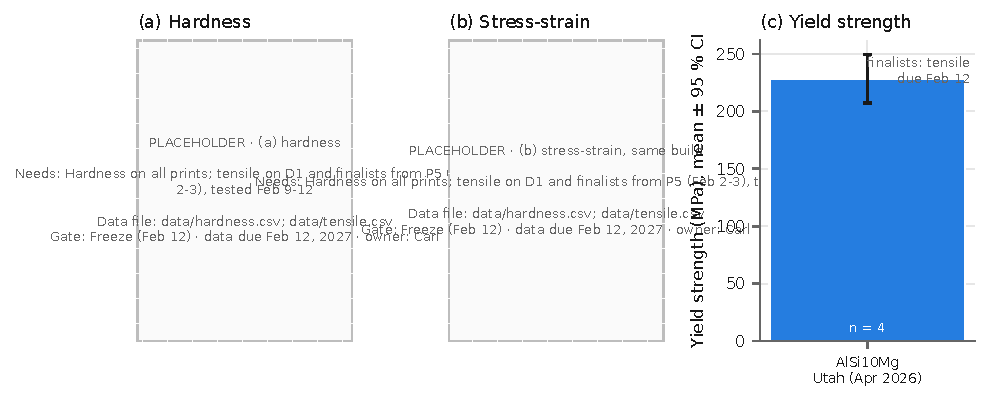
\includegraphics[width=\textwidth]{figures/fig5-mechanical.pdf}
  \caption{Strength and ductility. (a) Hardness \placeholder{of every printed composition}. (b) Stress--strain curves \placeholder{of the finalists and \AlSi from the same build}. (c) Yield strength, mean and 95\% confidence interval; the \AlSi bar is the April 2026 Utah build (as built, as-printed surfaces, horizontal, $n=\InhouseN$).}
  \label{fig:mech}
\end{figure}

\subsection{Corrosion}
\placeholder{Data due 12 Feb 2027 (Fig.~\ref{fig:corr}).}

\begin{figure}[tbp]
  \centering
  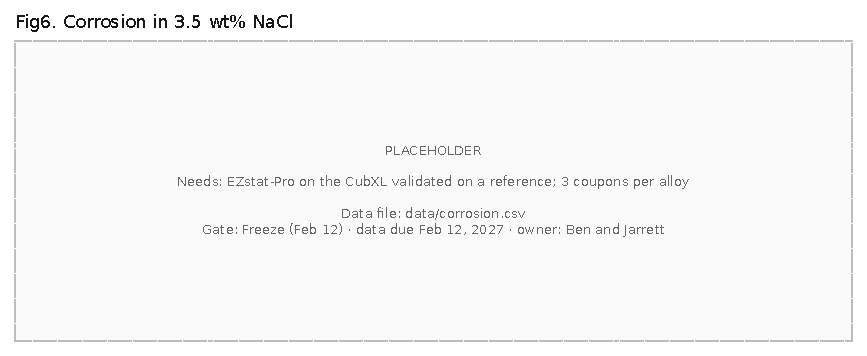
\includegraphics[width=\textwidth]{figures/fig6-corrosion.pdf}
  \caption{Corrosion in \SI{3.5}{wt\%} NaCl. \placeholder{(a) Polarization curves; (b) corrosion potential, corrosion current density and pitting potential.}}
  \label{fig:corr}
\end{figure}

\subsection{Independent verification}
\placeholder{Data due 19 Feb 2027 (Table~\ref{tab:verification}).}

\begin{table}[tbp]
  \centering\footnotesize
  \caption{Composition of the finalists measured in-house and by an outside laboratory. \placeholder{Filled from data/composition.csv when the outside reports arrive (due 19 Feb 2027).}}
  \label{tab:verification}
  \begin{tabular}{@{}llllll@{}}
    \toprule
    Alloy & Element & Target & EDS, in-house & Outside lab (method) & Difference \\
     & & (wt\%) & (wt\%) & (wt\%) & (wt\%) \\
    \midrule
    \multicolumn{6}{@{}l}{\placeholder{No outside laboratory contracted yet (risks.md, R8).}} \\
    \bottomrule
  \end{tabular}
\end{table}

% =============================================================================
\section{Comparison with \AlSi and \Scal}
\label{sec:benchmark}

\subsection{What the datasheets say}

Vendor datasheets give the properties that most readers will compare a new alloy with (Table~\ref{tab:benchmarks}, Fig.~\ref{fig:map}a).
As-built \AlSi reaches \SIrange{233}{300}{MPa} yield strength and \SIrange{450}{470}{MPa} tensile strength with \SIrange{5}{10.2}{\%} elongation on machined bars printed at \SI{30}{\micro m} layers~\cite{ds_eos,ds_nikon}.
Heat treatment trades strength for ductility: after a T6 treatment the yield strength is \SIrange{250}{260}{MPa} and the elongation 11\%, but the tensile strength falls to \SIrange{310}{320}{MPa}~\cite{ds_eos}; after a stress relief at \SI{285}{\celsius} the yield strength is \SI{165}{MPa}~\cite{ds_nikon}.
Unmachined vertical bars, closer to a printed part's as-built surfaces, average 3\% elongation, with a minimum of 1\%~\cite{ds_nikon}.
\Scal is about as strong as \AlSi as built (\SIrange{275}{295}{MPa}) but far more ductile (22--23\%), and after a direct age at \SI{325}{\celsius} for \SI{4}{h} it reaches \SIrange{465}{500}{MPa} yield strength with \SIrange{11.5}{15.8}{\%} elongation~\cite{ds_colibrium,ds_3dsystems}.


\subsection{\AlSi printed and tested the way the candidates are}

Datasheet values are each vendor's results on its own tuned parameters and machined specimens; they are not design allowables and they are not what a sub-size specimen with as-printed surfaces gives.
\AlSi printed for this work on the Aconity MIDI at the University of Utah from commercial gas-atomized powder, and tested as built with as-printed surfaces in the horizontal orientation, gave \InhouseYS~$\pm$~\InhouseYSsd~MPa yield strength, \InhouseUTS~$\pm$~\InhouseUTSsd~MPa tensile strength and \InhouseEL~$\pm$~\InhouseELsd\% elongation ($n=\InhouseN$; Table~\ref{tab:benchmarks}).
That is about \InhouseYSpctEOS\% of the EOS horizontal yield strength, \InhouseUTSpctEOS\% of its tensile strength and less than half its elongation (\InhouseEL{} against 10.2\%)~\cite{ds_eos}.
These April tests also predate the campaign's test method: strain came from the frame's own channel rather than an extensometer, three of the four valid tests gave elastic slopes of 29--49~GPa instead of about 70~GPa, elongation came from the same channel, and the crosshead rates were faster than ASTM E8/E8M allows while yield is measured. Their yield strengths are uncertain by up to about 30~MPa, and the comparator, including the \InhouseEL\% elongation threshold, is provisional until \AlSi is re-tested in the finalists' build.
The closest datasheet row is Nikon's unmachined (near-net-shape) bar, the only one with as-printed surfaces~\cite{ds_nikon}.
A candidate printed and tested in the same way as our specimens therefore has to be compared with our \AlSi, not with the datasheets.
Under the rule of Section~\ref{sec:stats}, with $n = \InhouseN$ for \AlSi (95\% confidence half-width \InhouseYShw~MPa), a candidate's mean yield strength must exceed \YSbar~MPa plus its own confidence half-width, about 270--280~MPa for three or four specimens with a similar spread, at an elongation of at least \InhouseEL\%. Such an alloy would still sit below the strongest machined as-built datasheet row (\SI{300}{MPa}), so a claim against our \AlSi is not a claim against the datasheets.
\note{This comparator is provisional: the April strain channel was unreliable for three of the four valid tests, and the powder was commercial. The finalists' build will contain both commercial and in-house \AlSi-type powder, with an extensometer, and those values replace these.}

\subsection{Scandium-free alloys that are already stronger than \AlSi}

Scandium-free alloys already sit between \AlSi and \Scal (Fig.~\ref{fig:map}a, grey markers).
On their vendors' datasheets, a directly aged Al--Mn--Cr--Zr powder reaches \SIrange{355}{370}{MPa} yield strength with \SIrange{12}{16}{\%} elongation~\cite{ds_hoganas}, a directly aged Al--Mg--Zr--Mn powder \SIrange{380}{385}{MPa} with 13--14.5\%~\cite{ds_al5x1}, and a heat-treated Al--Fe--Zr powder about \SI{300}{MPa} with 10--12\%~\cite{ds_cp1}; silver-bearing Al--Cu--Mg alloys reach \SIrange{350}{385}{MPa} as built and \SIrange{390}{460}{MPa} after a T7 or T4 treatment~\cite{ds_al2139,ds_a20x}, and a Zr-modified 7xxx alloy \SIrange{490}{585}{MPa} after hot isostatic pressing and heat treatment~\cite{ds_7a77}.
In the peer-reviewed literature, Al--Mn--Cr--Zr--Mg reached \SI{390}{MPa} as built with 17\% elongation~\cite{almncrzr2024}, Al--Mg--Zr \SIrange{350}{353}{MPa} after peak aging with 17--19\%~\cite{croteau2018}, Al--Mg--Mn--Er--Zr \SI{440}{MPa} after aging with 15.5\%~\cite{almgmnerzr2022}, Al--Fe--Mg--Zr \SI{376}{MPa} after aging with 11\%~\cite{alfezr2025}, and a tailored Al--Si--Mg alloy \SIrange{270}{417}{MPa} as built, depending on plate temperature and machine~\cite{alsimg2020}.
\note{Checked against the sources on 27 Nov 2026 (data/literature-alloys.csv, read\_by column). Still unverified: the as-built Al--Mg--Mn--Er--Zr row and its exact Zr content, and the as-built elongation of Al--Fe--Mg--Zr (full texts blocked).}
Being stronger than \AlSi without scandium is therefore not new in itself.
What the literature does not settle is how these alloys compare on critical-mineral burden, since each replaces scandium with several weight percent of Mn, Cr, Zr, Mg or rare earths, and how they compare with \AlSi printed and tested the same way.
A new alloy from this campaign is a contribution only if it sits beyond these alloys on strength against burden (Fig.~\ref{fig:map}b), not merely beyond \AlSi.

\subsection{Critical-mineral burden of the benchmarks}

Every element in the two benchmarks is on the final 2025 list~\cite{fr2025}, so the question is how much of each they carry, weighted by how exposed its supply is (Table~\ref{tab:compositions}).
On the import-weighted burden of Eq.~\ref{eq:burden}, \AlSi carries \BAlSinirlo--\BAlSinirhi~wt\% and \Scal \BScalnirlo--\BScalnirhi~wt\%; the ranges come from the reliances that USGS gives only as bounds~\cite{usgs2026}.
Most of \Scal's burden is its magnesium, not its \ScalSc~wt\% scandium, and most of \AlSi's is its 10~wt\% silicon. The two intervals overlap, but at their midpoints \AlSi scores higher.
On raw-material cost the order reverses: the critical additions in \Scal cost about \BScalcost~USD per kilogram of alloy, almost all of it scandium, against \BAlSicost~USD for \AlSi~\cite{usgs2026}. Priced through an Al--2Sc master alloy (30~USD per kilogram of master alloy) instead of the metal, the master alloy needed for \ScalSc~wt\% scandium still costs about \ScalMasterCost~USD per kilogram of \Scal~\cite{usgs2026sc}.
The premise that \AlSi carries fewer critical minerals than \Scal therefore holds for cost and for scandium, but not clearly for import-weighted mass.

The same split runs through the scandium-free alloys (Fig.~\ref{fig:map}b; Supplementary Fig.~S1).
On cost, with scandium priced as metal, all of them except the two silver-bearing Al--Cu--Mg alloys are at least \CostRedMinNonAg\% below \Scal (at least \CostRedMinMaster\% with scandium priced through the master alloy), and the silver-bearing ones are \CostRedAgLo--\CostRedAgHi\% below, so ``less than \Scal'' hardly tells them apart.
On import-weighted mass, the Mn-rich alloy that seed S1 reproduces sits above \Scal's interval (S1 at \BSonenirlo--\BSonenirhi~wt\%), the commercial Al--Mn--Cr--Zr grade sits inside it, and Al--Fe--Zr, Al--Fe--Mg--Zr and Al--Mg--Zr alloys sit well below it and, after aging, report higher yield strengths than our as-built \AlSi~\cite{ds_cp1,alfezr2025,ds_al5x1,croteau2018}.
Of the \NLit{} scandium-free comparators in Fig.~\ref{fig:map}b, \NLitRegionMid{} already sit in the shaded region at the midpoint of their burden, and \NLitRegionRobust{} even at the top of their burden interval. These are their reported values, mostly on machined specimens from tuned processes, so they are not like-for-like with our \AlSi; against the strongest machined \AlSi datasheet row instead (\SI{300}{MPa}), \NLitRegionMidDS{} and \NLitRegionRobustDS{} remain.
A campaign alloy therefore counts as a discovery only if it lies beyond these alloys on strength against burden, measured the same way and under the metric fixed in advance.
\note{This is the main risk to the paper's claim (risks.md, R1--R2). Sterling: pick the primary metric now. Under $B_\mathrm{NIR}$, steer the screen toward Fe-, Zr- and Mg-lean families (S2, O1) and away from Mn-rich ones (S1, O3); under $B_\mathrm{cost}$, any Sc-free alloy passes and the claim rests on strength alone.}



% =============================================================================
\section{Limitations}
\label{sec:limits}

\placeholder{Write at the data freeze.} All properties are at room temperature; elevated-temperature and cryogenic tests, fatigue and fracture toughness were outside the campaign. Specimens are sub-size, from one machine and, for most alloys, one build. Powder from ultrasonic atomization differs from commercial gas-atomized powder in size distribution and oxygen content, which is why the comparison with \AlSi uses both powder routes. The burden metric depends on 2025 import data and prices, and Supplementary Section~S3 shows how the ranking changes with the metric. None of this is qualification: the comparison is not a test against the \AlSi part specification~\cite{astm_f3318}, and a flight part would also need a qualified material process and a property suite under a standard such as NASA-STD-6030~\cite{nasa6030}.

\section{Conclusions}
\placeholder{Write at G4.}

% =============================================================================
\section*{Data availability}
\sloppy
The data behind every figure and table (run records, powder, print, density, hardness, tensile and corrosion data, and outside laboratory reports, with analysts' names and signatures removed) are in the project repository, \url{https://github.com/vertical-cloud-lab/digital-alloy-lab}, under \nolinkurl{al-campaign-paper/data/}, and will be archived with a DOI at \placeholder{Zenodo, DOI to be minted at submission}. Vendor datasheet values are cited to their sources and are not redistributed.

\section*{Code availability}
The scripts that compute the critical-mineral burden and draw every figure and table from the data are in \nolinkurl{al-campaign-paper/scripts/} in the same repository, released under the repository's MIT licence, and archived with the data.

\fussy
\section*{CRediT authorship contribution statement}
\placeholder{Draft from the campaign's stream leads (\#256); each author to confirm their own.} Gage Erickson: investigation (atomization), resources. Ronnie Guymon: investigation (powder characterization, SEM--EDS), data curation. Carl Robison: investigation (printing, mechanical testing). Xavier Zaitzeff: software, formal analysis (CALPHAD screening, optimization). \placeholder{Ben, Jarrett: investigation (corrosion). Paul: resources (charge preparation). University of Utah collaborators: resources (printing).} Sterling G. Baird: conceptualization, methodology, supervision, funding acquisition, writing -- original draft, writing -- review and editing.

\section*{Declaration of competing interest}
\placeholder{To confirm with each author.}

\section*{Declaration of generative AI and AI-assisted technologies in the writing process}
\placeholder{Confirm against the chosen journal's policy. Elsevier's template:} During the preparation of this work the authors used Claude (Anthropic) to draft text, compile and check references, and write the analysis scripts. After using this tool, the authors reviewed and edited the content as needed and take full responsibility for the content of the published article.

\section*{Acknowledgements}
\placeholder{University of Utah Metal 3D Printing Core Facility; funding.}

\bibliographystyle{elsarticle-num}
\bibliography{references}

\end{document}
